\chapter{数值模拟结果与分析}
本次实验共运行了 9 个样例,航行体入水角度分别为 $90 ^\circ$ 垂直入水以及 $60 ^\circ$ 和$45 ^\circ$入水。所有样例的均运行 2 秒,并保留了各运行时段的动力学状态。

\section{稳定的波浪场结果}
在进行完网格划分,边界条件设计,引入动量源项消波法之后,通过合适的数值方法,成功模拟了稳定的波浪场结果。下面为波浪传播某时刻的密度图,压强分布图和速度分布图。本文的算例是三维算例,但为了更直观地展示计算的结果,选取了在 $z$ 方向为对称轴的剖面进行图形的绘制。如无特殊说明,本文中展示的二维流场图形(如密度图,流场速度图等)均为在 $z$ 方向对称轴位置的流场结果。

\begin{figure}[!htp]
  \centering
  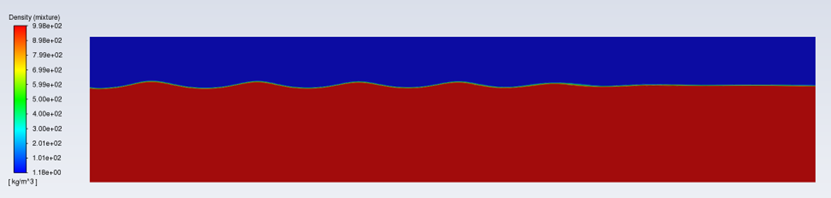
\includegraphics[]{fig/wave_density.png}
  \caption{波浪场密度($\rho$)图}
\end{figure}

波浪场压强分布如图\ref{fig:wave_pressure}所示,可以看到,空气和水体之间的压力区分明显,液体区域随深度增加压强逐渐升高。
\begin{figure}[!htp]
  \centering
  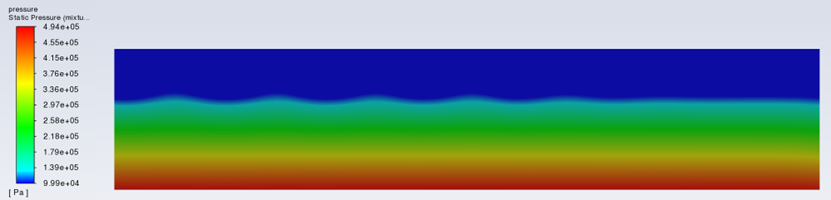
\includegraphics[]{fig/wave_pressure.png}
  \caption{波浪场压强($p$)分布图}
  \label{fig:wave_pressure}
\end{figure}

波浪场速度分布图如图\ref{fig:wave_u},\ref{fig:wave_v}所示,在工作区呈现典型的波浪场速度分布特征,在消波区存在一定的$u$分布,也符合动量源项消波法的结果。
\begin{figure}[!htp]
  \centering
  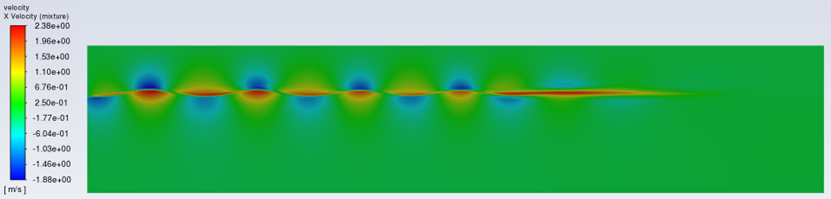
\includegraphics[]{fig/wave_u.png}
  \caption{波浪场$x$方向速度($u$)分布图}
  \label{fig:wave_u}
\end{figure}
\begin{figure}[!htp]
  \centering
  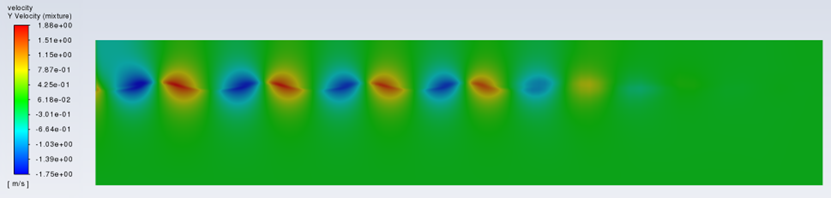
\includegraphics[]{fig/wave_v.png}
  \caption{波浪场$y$方向速度($v$)分布图}
  \label{fig:wave_v}
\end{figure}

\section{不同入水阶段的密度分布}
在考虑并应用 VOF 捕捉方法和重叠网格技术后,可以顺利地进行入水数值模拟实验。数值模拟实验共进行 $t_{\max} = 2s$。以下是入射倾角为 $45^\circ$ 时,运行 $0s$、$0.5$、$0.7s$、$0.9s$、$2.0s$ 的局部密度图。

\begin{figure}[!htp]
  \centering
  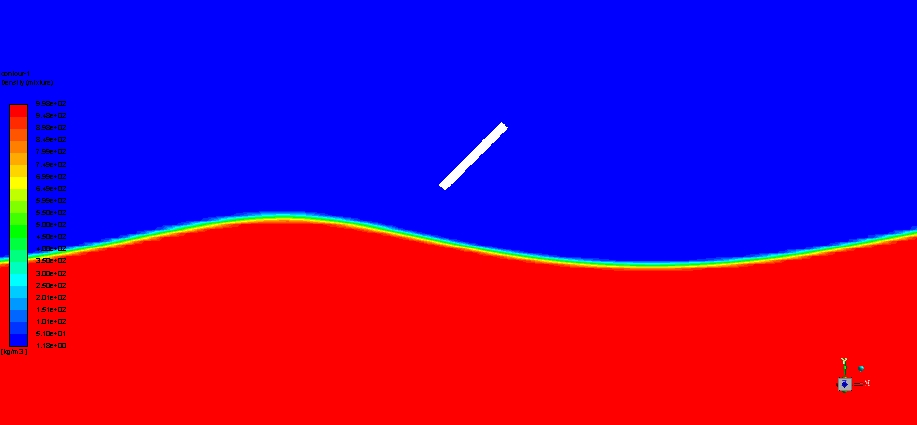
\includegraphics[width=0.5\textwidth]{fig/WaterEntry-AOA45-1-0.jpg}
  \caption{$t=0s$时局部密度图} 
\end{figure}

\begin{figure}[!htp]
  \centering
  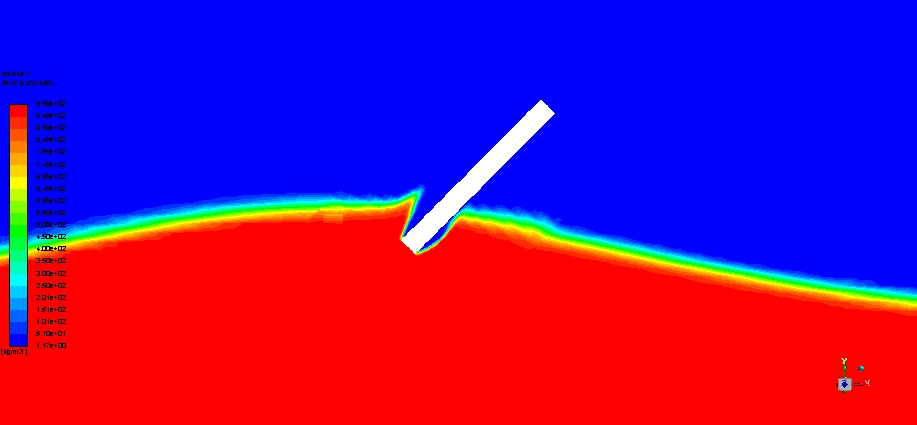
\includegraphics[width=0.5\textwidth]{fig/WaterEntry-AOA45-1-0_5.jpg}
  \caption{$t=0.5s$时局部密度图}
\end{figure}

\begin{figure}[!htp]
  \centering
  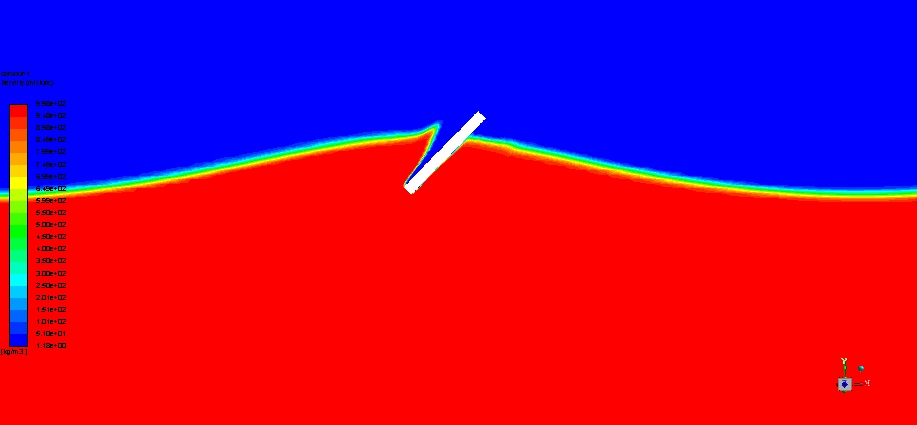
\includegraphics[width=0.5\textwidth]{fig/WaterEntry-AOA45-1-0_7.jpg}
  \caption*{$t=0.7s$时局部密度图} 
\end{figure}

\begin{figure}[!htp]
  \centering
  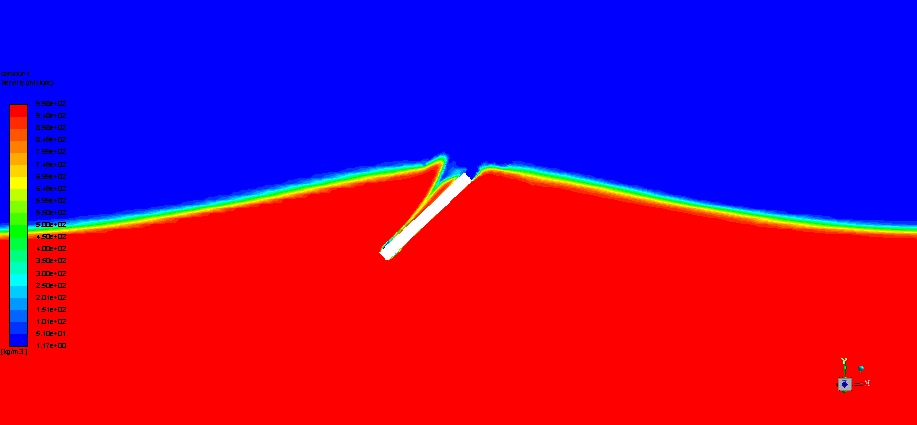
\includegraphics[width=0.5\textwidth]{fig/WaterEntry-AOA45-1-0_9.jpg}
  \caption{$t=0.9s$时局部密度图} 
\end{figure}

\begin{figure}[!htp]
  \centering
  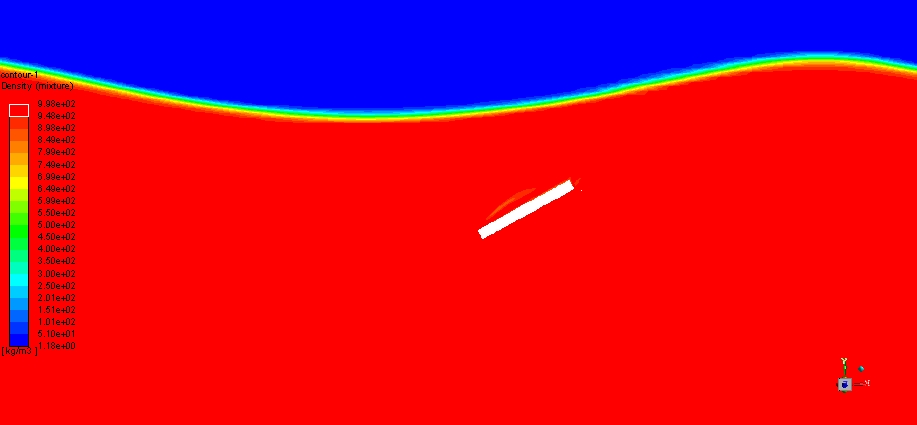
\includegraphics[width=0.5\textwidth]{fig/WaterEntry-AOA45-1-2_000000.jpg}
  \caption{$t=2.0s$时局部密度图} 
\end{figure}

可以看到入水过程发生了显著的空泡现象。将这些结果与理论分析和实验的结果进行对比,发现与实际符合良好,这也验证了模型的准确性。

\section{入水过程的流场状态细节分析}

为了更好地观察和描述入水过程中的现象,本文首先对入射角度与水面夹角为 $60^\circ$,$90 ^\circ$ 和 $45 ^\circ$ 的各一个算例(均为各入水角度的算例 3 )的入水过程的详细情况进行了分析,从而得到航行体进入波浪场时的一般情况。

\subsection{$60 ^\circ$入水条件下的入水过程流场状态细节}

本文首先对 $60 ^\circ$ 的算例进行了分析,如图\ref{fig:detail_d}所示。可以看到,从 $t = 0.3 s$航行体首次接触波浪场水面开始,大约总共进行了 $0.5 s$ 才使整个航行体全部没入波浪场中。航行体在进入波浪场中的同时,波浪场也在进行运动,在 $t= 0.3s$时,航行体与波浪场的接触点约在相位 $\varphi = \pi$ 左右,而当 $t = 0.8s$ 航行体全部进入水中时,前述位置下波浪场已经运行至 $\varphi = \pi / 2$ 的相位。在 $0.5s$ 的过程中,波浪场运行相位约为 $\pi / 2$,这也与实验中预先给定的 Stokes 波的参数相符合。入水过程中有非常明显的空泡现象。在航行体刚进入水面时,空泡出现在航行体的四周,且从头部至水面都有空泡。随着航行体的不断运行,右下侧的空泡逐渐坍缩,且航行体头部附近的空泡逐渐消失,空泡聚集在了航行体的尾部。在整个航行体运行期间,尽管航行体进入水下并引起了空泡已经扰动,但明显可以发现整个流场还保持非常稳定的波浪场状态。这得益于流场区域在 $z$ 轴方向具有比较大的深度,直径仅为 $0.5m$ 的航行体不会对具有持续波浪的流场产生使整体改变波浪状态的影响。

\begin{figure}[!htp]
  \centering

  \begin{subfigure}{0.25\textwidth}
    \centering
    \includegraphics[width = \textwidth]{fig/aoa60_60st/3d.jpg}
    \caption{$t = 0.3s$}
  \end{subfigure}
  \hspace{1cm}
  \begin{subfigure}{0.25\textwidth}
    \centering
    \includegraphics[width = \textwidth]{fig/aoa60_60st/4d.jpg}
    \caption{$t = 0.4s$}
  \end{subfigure}
  \hspace{1cm}
  \begin{subfigure}{0.25\textwidth}
    \centering
    \includegraphics[width = \textwidth]{fig/aoa60_60st/5d.jpg}
    \caption{$t = 0.5s$}
  \end{subfigure}

  \quad

  \begin{subfigure}{0.25\textwidth}
    \centering
    \includegraphics[width = \textwidth]{fig/aoa60_60st/6d.jpg}
    \caption{$t = 0.6s$}
  \end{subfigure}
  \hspace{1cm}
  \begin{subfigure}{0.25\textwidth}
    \centering
    \includegraphics[width = \textwidth]{fig/aoa60_60st/7d.jpg}
    \caption{$t = 0.7s$}
  \end{subfigure}
  \hspace{1cm}
  \begin{subfigure}{0.25\textwidth}
    \centering
    \includegraphics[width = \textwidth]{fig/aoa60_60st/8d.jpg}
    \caption{$t = 0.8s$}
  \end{subfigure}

  \quad 

  \begin{subfigure}{0.25\textwidth}
    \centering
    \includegraphics[width = \textwidth]{fig/aoa60_60st/12d.jpg}
    \caption{$t = 1.2s$}
  \end{subfigure}
  \hspace{1cm}
  \begin{subfigure}{0.25\textwidth}
    \centering
    \includegraphics[width = \textwidth]{fig/aoa60_60st/16d.jpg}
    \caption{$t = 1.6s$}
  \end{subfigure}
  \hspace{1cm}
  \begin{subfigure}{0.25\textwidth}
    \centering
    \includegraphics[width = \textwidth]{fig/aoa60_60st/20d.jpg}
    \caption{$t = 2.0s$}
  \end{subfigure}

  \caption{$60^\circ$入水角度下第三个算例的密度场}
  \label{fig:detail_d}
\end{figure}

航行过程中的压力图如图\ref{fig:detail_p}所示,图b)至图f)的压力范围均取自 $0.8 \times 10^5 \sim 2 \times 10^5 \mathrm{Pa}$,而图a)的压力范围为$0.8 \times 10^5 \sim 4 \times 10^5 \mathrm{Pa}$,所以会使图a)的背景场看起来与其他场不同。使用不同的压力范围取值是因为图a)接触前端的压力很大。可以看到背景波浪场中,空气部分由于连接大气,其压强保持在 $10^5 \mathrm{Pa}$ 左右,而水内部则随着深度的增加压力逐渐增加。本次数值实验采用的航行体为圆柱体,可以明显看到其前端受到的阻力很大。前端压力最大的情况出现在刚接触水面的时候,在本算例中到达了接近 $4 \times 10^5 \mathrm{Pa}$ 的压力。前端压力在物体刚接触到水面时迅速提升并达到最大值,在航行体前端已经浸入水面后,其前端压力依旧较高,且前端一定区域内都受高压影响,但相对于刚接触水面时保持相对较少水平,且在航行过程中没有太大变化。航行体两侧存在一定的低压区,低压区发生在存在空泡的区域,在 $t = 0.4s$ 和 $t = 0.5s$ 空泡时非常明显,这与空泡现象的理论分析和常规实验结果相一致。航行体前端的侧面是航行体压力最低的区域。在 $t= 0.6s$ 和 $t = 0.7s$ 时航行体右侧空泡已接近消失,右侧局部压力不降反升。

\begin{figure}[!htp]
  \centering

  \begin{subfigure}{0.25\textwidth}
    \centering
    \includegraphics[width = \textwidth]{fig/aoa60_60st/3p.jpg}
    \caption{$t = 0.3s$}
  \end{subfigure}
  \hspace{1cm}
  \begin{subfigure}{0.25\textwidth}
    \centering
    \includegraphics[width = \textwidth]{fig/aoa60_60st/4p.jpg}
    \caption{$t = 0.4s$}
  \end{subfigure}
  \hspace{1cm}
  \begin{subfigure}{0.25\textwidth}
    \centering
    \includegraphics[width = \textwidth]{fig/aoa60_60st/5p.jpg}
    \caption{$t = 0.5s$}
  \end{subfigure}

  \quad

  \begin{subfigure}{0.25\textwidth}
    \centering
    \includegraphics[width = \textwidth]{fig/aoa60_60st/6p.jpg}
    \caption{$t = 0.6s$}
  \end{subfigure}
  \hspace{1cm}
  \begin{subfigure}{0.25\textwidth}
    \centering
    \includegraphics[width = \textwidth]{fig/aoa60_60st/7p.jpg}
    \caption{$t = 0.7s$}
  \end{subfigure}
  \hspace{1cm}
  \begin{subfigure}{0.25\textwidth}
    \centering
    \includegraphics[width = \textwidth]{fig/aoa60_60st/8p.jpg}
    \caption{$t = 0.8s$}
  \end{subfigure}

  \quad 

  \begin{subfigure}{0.25\textwidth}
    \centering
    \includegraphics[width = \textwidth]{fig/aoa60_60st/12p.jpg}
    \caption{$t = 1.2s$}
  \end{subfigure}
  \hspace{1cm}
  \begin{subfigure}{0.25\textwidth}
    \centering
    \includegraphics[width = \textwidth]{fig/aoa60_60st/16p.jpg}
    \caption{$t = 1.6s$}
  \end{subfigure}
  \hspace{1cm}
  \begin{subfigure}{0.25\textwidth}
    \centering
    \includegraphics[width = \textwidth]{fig/aoa60_60st/20p.jpg}
    \caption{$t = 2.0s$}
  \end{subfigure}

  \caption{$60^\circ$入水角度下第三个算例的压力场}
  \label{fig:detail_p}
\end{figure}

航行过程中的水平方向速度$u$图和垂直方向速度 $v$ 图如图\ref{fig:detail_u}和图\ref{fig:detail_v}所示。这些图的坐标刻度都不相同。通过比较各流场时刻的速度分布,可以发现整个背景场的速度分布与二阶 Stokes 波的速度分布符合地很好。尽管受本身时变的波浪背景场的影响,但航行体附近的流场速度场依旧有许多规律,并且与一般的流体力学理论相符合。航行体与接触的流体之间形成固壁边界条件,其前端和尾端都是圆截面,在航行过程中受到较大的阻力。其前端前方和尾端后方的速度场都是与航行体的运行速度方向相一致的。在航行体附近的空泡区域,其运动速度比较大,且速度方向平行于航行体边缘的方向。在 $t = 0.4s$ 和 $t = 0.5s$ 的时刻在航行体的前端空泡处具有逆时针方向的速度。在 $t = 0.6 \sim 0.8 s$ 时,航行体右后方的空泡转移并消失,空泡转移至航行体左上侧,流场运动方向与航行体运动方向相反。 


\begin{figure}[!htp]
  \centering

  \begin{subfigure}{0.25\textwidth}
    \centering
    \includegraphics[width = \textwidth]{fig/aoa60_60st/3u.jpg}
    \caption{$t = 0.3s$}
  \end{subfigure}
  \hspace{1cm}
  \begin{subfigure}{0.25\textwidth}
    \centering
    \includegraphics[width = \textwidth]{fig/aoa60_60st/4u.jpg}
    \caption{$t = 0.4s$}
  \end{subfigure}
  \hspace{1cm}
  \begin{subfigure}{0.25\textwidth}
    \centering
    \includegraphics[width = \textwidth]{fig/aoa60_60st/5u.jpg}
    \caption{$t = 0.5s$}
  \end{subfigure}

  \quad

  \begin{subfigure}{0.25\textwidth}
    \centering
    \includegraphics[width = \textwidth]{fig/aoa60_60st/6u.jpg}
    \caption{$t = 0.6s$}
  \end{subfigure}
  \hspace{1cm}
  \begin{subfigure}{0.25\textwidth}
    \centering
    \includegraphics[width = \textwidth]{fig/aoa60_60st/7u.jpg}
    \caption{$t = 0.7s$}
  \end{subfigure}
  \hspace{1cm}
  \begin{subfigure}{0.25\textwidth}
    \centering
    \includegraphics[width = \textwidth]{fig/aoa60_60st/8u.jpg}
    \caption{$t = 0.8s$}
  \end{subfigure}

  \quad 

  \begin{subfigure}{0.25\textwidth}
    \centering
    \includegraphics[width = \textwidth]{fig/aoa60_60st/12u.jpg}
    \caption{$t = 1.2s$}
  \end{subfigure}
  \hspace{1cm}
  \begin{subfigure}{0.25\textwidth}
    \centering
    \includegraphics[width = \textwidth]{fig/aoa60_60st/16u.jpg}
    \caption{$t = 1.6s$}
  \end{subfigure}
  \hspace{1cm}
  \begin{subfigure}{0.25\textwidth}
    \centering
    \includegraphics[width = \textwidth]{fig/aoa60_60st/20u.jpg}
    \caption{$t = 2.0s$}
  \end{subfigure}

  \caption{$60^\circ$入水角度下第三个算例的水平速度场}
  \label{fig:detail_u}
\end{figure}
\begin{figure}[!htp]
  \centering

  \begin{subfigure}{0.25\textwidth}
    \centering
    \includegraphics[width = \textwidth]{fig/aoa60_60st/3v.jpg}
    \caption{$t = 0.3s$}
  \end{subfigure}
  \hspace{1cm}
  \begin{subfigure}{0.25\textwidth}
    \centering
    \includegraphics[width = \textwidth]{fig/aoa60_60st/4v.jpg}
    \caption{$t = 0.4s$}
  \end{subfigure}
  \hspace{1cm}
  \begin{subfigure}{0.25\textwidth}
    \centering
    \includegraphics[width = \textwidth]{fig/aoa60_60st/5v.jpg}
    \caption{$t = 0.5s$}
  \end{subfigure}

  \quad

  \begin{subfigure}{0.25\textwidth}
    \centering
    \includegraphics[width = \textwidth]{fig/aoa60_60st/6v.jpg}
    \caption{$t = 0.6s$}
  \end{subfigure}
  \hspace{1cm}
  \begin{subfigure}{0.25\textwidth}
    \centering
    \includegraphics[width = \textwidth]{fig/aoa60_60st/7v.jpg}
    \caption{$t = 0.7s$}
  \end{subfigure}
  \hspace{1cm}
  \begin{subfigure}{0.25\textwidth}
    \centering
    \includegraphics[width = \textwidth]{fig/aoa60_60st/8v.jpg}
    \caption{$t = 0.8s$}
  \end{subfigure}

  \quad 

  \begin{subfigure}{0.25\textwidth}
    \centering
    \includegraphics[width = \textwidth]{fig/aoa60_60st/12v.jpg}
    \caption{$t = 1.2s$}
  \end{subfigure}
  \hspace{1cm}
  \begin{subfigure}{0.25\textwidth}
    \centering
    \includegraphics[width = \textwidth]{fig/aoa60_60st/16v.jpg}
    \caption{$t = 1.6s$}
  \end{subfigure}
  \hspace{1cm}
  \begin{subfigure}{0.25\textwidth}
    \centering
    \includegraphics[width = \textwidth]{fig/aoa60_60st/20v.jpg}
    \caption{$t = 2.0s$}
  \end{subfigure}

  \caption{$60^\circ$入水角度下第三个算例的竖直速度场}
  \label{fig:detail_v}
\end{figure}

上面的分析基于航行体入射角度为 $60 ^\circ$ 的情形,航行体入射角度为 $45 ^\circ$ 的情形中,其动力学特性一定程度上与 $60 ^\circ$ 的相同。然而,当航行体入射角度为 $90 ^\circ$ 的情形下,其许多情况与具有较大倾斜角度的入射是不同的,因此对于垂直入射的情形,这里也打算对其进行分析。

\subsection{$90 ^\circ$入水条件下的入水过程流场状态细节}

航行体在 $90 ^\circ$ 第三个算例下的入射的密度场如图\ref{fig:detail_90_d}所示。本次航行的入水过程大概发生在 $t = 0.25s$ 时,大约在 $t = 0.75s$ 时完成入水过程。在与前一次的入水过程相似,在入水过程中具有明显的空泡现象,并且空泡现象持续地更加持久在本次入水的过程中,更多的空泡出现在航行体的右侧,这与倾斜入水时的结果略有不同,导致这一现象的很重要的原因是初始速度场的方向向右,导致左侧的空泡会更快地消失。航行体在航行的过程中入射角逐渐减小。

\begin{figure}[!htp]
  \centering

  \begin{subfigure}{0.25\textwidth}
    \centering
    \includegraphics[width = \textwidth]{fig/aoa90_60st/2d.jpg}
    \caption{$t = 0.25s$}
  \end{subfigure}
  \hspace{1cm}
  \begin{subfigure}{0.25\textwidth}
    \centering
    \includegraphics[width = \textwidth]{fig/aoa90_60st/3d.jpg}
    \caption{$t = 0.35s$}
  \end{subfigure}
  \hspace{1cm}
  \begin{subfigure}{0.25\textwidth}
    \centering
    \includegraphics[width = \textwidth]{fig/aoa90_60st/4d.jpg}
    \caption{$t = 0.45s$}
  \end{subfigure}

  \quad

  \begin{subfigure}{0.25\textwidth}
    \centering
    \includegraphics[width = \textwidth]{fig/aoa90_60st/5d.jpg}
    \caption{$t = 0.55s$}
  \end{subfigure}
  \hspace{1cm}
  \begin{subfigure}{0.25\textwidth}
    \centering
    \includegraphics[width = \textwidth]{fig/aoa90_60st/6d.jpg}
    \caption{$t = 0.65s$}
  \end{subfigure}
  \hspace{1cm}
  \begin{subfigure}{0.25\textwidth}
    \centering
    \includegraphics[width = \textwidth]{fig/aoa90_60st/7d.jpg}
    \caption{$t = 0.75s$}
  \end{subfigure}

  \quad

  \begin{subfigure}{0.25\textwidth}
    \centering
    \includegraphics[width = \textwidth]{fig/aoa90_60st/12d.jpg}
    \caption{$t = 1.20s$}
  \end{subfigure}
  \hspace{1cm}
  \begin{subfigure}{0.25\textwidth}
    \centering
    \includegraphics[width = \textwidth]{fig/aoa90_60st/16d.jpg}
    \caption{$t = 1.60s$}
  \end{subfigure}
  \hspace{1cm}
  \begin{subfigure}{0.25\textwidth}
    \centering
    \includegraphics[width = \textwidth]{fig/aoa90_60st/20d.jpg}
    \caption{$t = 2.00s$}
  \end{subfigure}

  \caption{$90^\circ$入水角度下第三个算例的密度场}
  \label{fig:detail_90_d}
\end{figure}

航行过程的压力场如图\ref{fig:detail_90_p}所示。在 $t = 0.25s$ 时,航行体刚刚接触水面的一部分,受到的压力较小。随后的行进过程中,航行体两侧的空泡部分压力较小,航行体前端部分受到的压力较大,与前述的 $60^\circ$ 时的压力分布较为相似。

\begin{figure}[!htp]
  \centering

  \begin{subfigure}{0.25\textwidth}
    \centering
    \includegraphics[width = \textwidth]{fig/aoa90_60st/2p.jpg}
    \caption{$t = 0.25s$}
  \end{subfigure}
  \hspace{1cm}
  \begin{subfigure}{0.25\textwidth}
    \centering
    \includegraphics[width = \textwidth]{fig/aoa90_60st/3p.jpg}
    \caption{$t = 0.35s$}
  \end{subfigure}
  \hspace{1cm}
  \begin{subfigure}{0.25\textwidth}
    \centering
    \includegraphics[width = \textwidth]{fig/aoa90_60st/4p.jpg}
    \caption{$t = 0.45s$}
  \end{subfigure}

  \quad

  \begin{subfigure}{0.25\textwidth}
    \centering
    \includegraphics[width = \textwidth]{fig/aoa90_60st/5p.jpg}
    \caption{$t = 0.55s$}
  \end{subfigure}
  \hspace{1cm}
  \begin{subfigure}{0.25\textwidth}
    \centering
    \includegraphics[width = \textwidth]{fig/aoa90_60st/6p.jpg}
    \caption{$t = 0.65s$}
  \end{subfigure}
  \hspace{1cm}
  \begin{subfigure}{0.25\textwidth}
    \centering
    \includegraphics[width = \textwidth]{fig/aoa90_60st/7p.jpg}
    \caption{$t = 0.75s$}
  \end{subfigure}

  \quad

  \begin{subfigure}{0.25\textwidth}
    \centering
    \includegraphics[width = \textwidth]{fig/aoa90_60st/12p.jpg}
    \caption{$t = 1.20s$}
  \end{subfigure}
  \hspace{1cm}
  \begin{subfigure}{0.25\textwidth}
    \centering
    \includegraphics[width = \textwidth]{fig/aoa90_60st/16p.jpg}
    \caption{$t = 1.60s$}
  \end{subfigure}
  \hspace{1cm}
  \begin{subfigure}{0.25\textwidth}
    \centering
    \includegraphics[width = \textwidth]{fig/aoa90_60st/20p.jpg}
    \caption{$t = 2.00s$}
  \end{subfigure}

  \caption{$90^\circ$入水角度下第三个算例的压力场}
  \label{fig:detail_90_p}
\end{figure}

$90^\circ$ 下航行体运行的速度场如图\ref{fig:detail_90_u}和图\ref{fig:detail_90_v}所示,在 $t = 0.35s$ 和 $t = 0.45s$ 的入水阶段前段,航行体前端两侧部分流场速度向外,这是由于航行体前进过程前端对其的挤压造成的。航行体前进过程中的空泡内流体运动速度较快,运动方向向远离航行的方向以及与航行体运动方向相反。

\begin{figure}[!htp]
  \centering

  \begin{subfigure}{0.25\textwidth}
    \centering
    \includegraphics[width = \textwidth]{fig/aoa90_60st/2u.jpg}
    \caption{$t = 0.25s$}
  \end{subfigure}
  \hspace{1cm}
  \begin{subfigure}{0.25\textwidth}
    \centering
    \includegraphics[width = \textwidth]{fig/aoa90_60st/3u.jpg}
    \caption{$t = 0.35s$}
  \end{subfigure}
  \hspace{1cm}
  \begin{subfigure}{0.25\textwidth}
    \centering
    \includegraphics[width = \textwidth]{fig/aoa90_60st/4u.jpg}
    \caption{$t = 0.45s$}
  \end{subfigure}

  \quad

  \begin{subfigure}{0.25\textwidth}
    \centering
    \includegraphics[width = \textwidth]{fig/aoa90_60st/5u.jpg}
    \caption{$t = 0.55s$}
  \end{subfigure}
  \hspace{1cm}
  \begin{subfigure}{0.25\textwidth}
    \centering
    \includegraphics[width = \textwidth]{fig/aoa90_60st/6u.jpg}
    \caption{$t = 0.65s$}
  \end{subfigure}
  \hspace{1cm}
  \begin{subfigure}{0.25\textwidth}
    \centering
    \includegraphics[width = \textwidth]{fig/aoa90_60st/7u.jpg}
    \caption{$t = 0.75s$}
  \end{subfigure}

  \quad

  \begin{subfigure}{0.25\textwidth}
    \centering
    \includegraphics[width = \textwidth]{fig/aoa90_60st/12u.jpg}
    \caption{$t = 1.20s$}
  \end{subfigure}
  \hspace{1cm}
  \begin{subfigure}{0.25\textwidth}
    \centering
    \includegraphics[width = \textwidth]{fig/aoa90_60st/16u.jpg}
    \caption{$t = 1.60s$}
  \end{subfigure}
  \hspace{1cm}
  \begin{subfigure}{0.25\textwidth}
    \centering
    \includegraphics[width = \textwidth]{fig/aoa90_60st/20u.jpg}
    \caption{$t = 2.00s$}
  \end{subfigure}

  \caption{$90^\circ$入水角度下第三个算例的水平速度场}
  \label{fig:detail_90_u}
\end{figure}

\begin{figure}[!htp]
  \centering

  \begin{subfigure}{0.25\textwidth}
    \centering
    \includegraphics[width = \textwidth]{fig/aoa90_60st/2v.jpg}
    \caption{$t = 0.25s$}
  \end{subfigure}
  \hspace{1cm}
  \begin{subfigure}{0.25\textwidth}
    \centering
    \includegraphics[width = \textwidth]{fig/aoa90_60st/3v.jpg}
    \caption{$t = 0.35s$}
  \end{subfigure}
  \hspace{1cm}
  \begin{subfigure}{0.25\textwidth}
    \centering
    \includegraphics[width = \textwidth]{fig/aoa90_60st/4v.jpg}
    \caption{$t = 0.45s$}
  \end{subfigure}

  \quad

  \begin{subfigure}{0.25\textwidth}
    \centering
    \includegraphics[width = \textwidth]{fig/aoa90_60st/5v.jpg}
    \caption{$t = 0.55s$}
  \end{subfigure}
  \hspace{1cm}
  \begin{subfigure}{0.25\textwidth}
    \centering
    \includegraphics[width = \textwidth]{fig/aoa90_60st/6v.jpg}
    \caption{$t = 0.65s$}
  \end{subfigure}
  \hspace{1cm}
  \begin{subfigure}{0.25\textwidth}
    \centering
    \includegraphics[width = \textwidth]{fig/aoa90_60st/7v.jpg}
    \caption{$t = 0.75s$}
  \end{subfigure}

  \quad

  \begin{subfigure}{0.25\textwidth}
    \centering
    \includegraphics[width = \textwidth]{fig/aoa90_60st/12v.jpg}
    \caption{$t = 1.20s$}
  \end{subfigure}
  \hspace{1cm}
  \begin{subfigure}{0.25\textwidth}
    \centering
    \includegraphics[width = \textwidth]{fig/aoa90_60st/16v.jpg}
    \caption{$t = 1.60s$}
  \end{subfigure}
  \hspace{1cm}
  \begin{subfigure}{0.25\textwidth}
    \centering
    \includegraphics[width = \textwidth]{fig/aoa90_60st/20v.jpg}
    \caption{$t = 2.00s$}
  \end{subfigure}

  \caption{$90^\circ$入水角度下第三个算例的竖直速度场}
  \label{fig:detail_90_v}
\end{figure}

\subsection{$45 ^\circ$入水条件下的入水过程流场状态细节}

$45 ^\circ$ 下的航行体的入水过程如图 \ref{fig:detail_45_d}, \ref{fig:detail_45_p},\ref{fig:detail_45_u},\ref{fig:detail_45_v} 所示,可以看到航行过程中空泡现象明显。航行体接触到水面后,航行体前端正侧受到很大的压力,而航行体前端两侧的压力有所下降。在存在空泡的流场区域,流体运动速度上升。

\begin{figure}[!htp]
  \centering

  \begin{subfigure}{0.25\textwidth}
    \centering
    \includegraphics[width = \textwidth]{fig/aoa45_60st/3d.jpg}
    \caption{$t = 0.3s$}
  \end{subfigure}
  \hspace{1cm}
  \begin{subfigure}{0.25\textwidth}
    \centering
    \includegraphics[width = \textwidth]{fig/aoa45_60st/4d.jpg}
    \caption{$t = 0.4s$}
  \end{subfigure}
  \hspace{1cm}
  \begin{subfigure}{0.25\textwidth}
    \centering
    \includegraphics[width = \textwidth]{fig/aoa45_60st/5d.jpg}
    \caption{$t = 0.5s$}
  \end{subfigure}

  \quad

  \begin{subfigure}{0.25\textwidth}
    \centering
    \includegraphics[width = \textwidth]{fig/aoa45_60st/6d.jpg}
    \caption{$t = 0.6s$}
  \end{subfigure}
  \hspace{1cm}
  \begin{subfigure}{0.25\textwidth}
    \centering
    \includegraphics[width = \textwidth]{fig/aoa45_60st/7d.jpg}
    \caption{$t = 0.7s$}
  \end{subfigure}
  \hspace{1cm}
  \begin{subfigure}{0.25\textwidth}
    \centering
    \includegraphics[width = \textwidth]{fig/aoa45_60st/8d.jpg}
    \caption{$t = 0.8s$}
  \end{subfigure}

  \quad 

  \begin{subfigure}{0.25\textwidth}
    \centering
    \includegraphics[width = \textwidth]{fig/aoa45_60st/12d.jpg}
    \caption{$t = 1.2s$}
  \end{subfigure}
  \hspace{1cm}
  \begin{subfigure}{0.25\textwidth}
    \centering
    \includegraphics[width = \textwidth]{fig/aoa45_60st/16d.jpg}
    \caption{$t = 1.6s$}
  \end{subfigure}
  \hspace{1cm}
  \begin{subfigure}{0.25\textwidth}
    \centering
    \includegraphics[width = \textwidth]{fig/aoa45_60st/20d.jpg}
    \caption{$t = 2.0s$}
  \end{subfigure}

  \caption{$45^\circ$入水角度下第三个算例的密度场}
  \label{fig:detail_45_d}
\end{figure}


\begin{figure}[!htp]
  \centering

  \begin{subfigure}{0.25\textwidth}
    \centering
    \includegraphics[width = \textwidth]{fig/aoa45_60st/3p.jpg}
    \caption{$t = 0.3s$}
  \end{subfigure}
  \hspace{1cm}
  \begin{subfigure}{0.25\textwidth}
    \centering
    \includegraphics[width = \textwidth]{fig/aoa45_60st/4p.jpg}
    \caption{$t = 0.4s$}
  \end{subfigure}
  \hspace{1cm}
  \begin{subfigure}{0.25\textwidth}
    \centering
    \includegraphics[width = \textwidth]{fig/aoa45_60st/5p.jpg}
    \caption{$t = 0.5s$}
  \end{subfigure}

  \quad

  \begin{subfigure}{0.25\textwidth}
    \centering
    \includegraphics[width = \textwidth]{fig/aoa45_60st/6p.jpg}
    \caption{$t = 0.6s$}
  \end{subfigure}
  \hspace{1cm}
  \begin{subfigure}{0.25\textwidth}
    \centering
    \includegraphics[width = \textwidth]{fig/aoa45_60st/7p.jpg}
    \caption{$t = 0.7s$}
  \end{subfigure}
  \hspace{1cm}
  \begin{subfigure}{0.25\textwidth}
    \centering
    \includegraphics[width = \textwidth]{fig/aoa45_60st/8p.jpg}
    \caption{$t = 0.8s$}
  \end{subfigure}

  \quad 

  \begin{subfigure}{0.25\textwidth}
    \centering
    \includegraphics[width = \textwidth]{fig/aoa45_60st/12p.jpg}
    \caption{$t = 1.2s$}
  \end{subfigure}
  \hspace{1cm}
  \begin{subfigure}{0.25\textwidth}
    \centering
    \includegraphics[width = \textwidth]{fig/aoa45_60st/16p.jpg}
    \caption{$t = 1.6s$}
  \end{subfigure}
  \hspace{1cm}
  \begin{subfigure}{0.25\textwidth}
    \centering
    \includegraphics[width = \textwidth]{fig/aoa45_60st/20p.jpg}
    \caption{$t = 2.0s$}
  \end{subfigure}

  \caption{$45^\circ$入水角度下第三个算例的压力场}
  \label{fig:detail_45_p}
\end{figure}

\begin{figure}[!htp]
  \centering

  \begin{subfigure}{0.25\textwidth}
    \centering
    \includegraphics[width = \textwidth]{fig/aoa45_60st/3u.jpg}
    \caption{$t = 0.3s$}
  \end{subfigure}
  \hspace{1cm}
  \begin{subfigure}{0.25\textwidth}
    \centering
    \includegraphics[width = \textwidth]{fig/aoa45_60st/4u.jpg}
    \caption{$t = 0.4s$}
  \end{subfigure}
  \hspace{1cm}
  \begin{subfigure}{0.25\textwidth}
    \centering
    \includegraphics[width = \textwidth]{fig/aoa45_60st/5u.jpg}
    \caption{$t = 0.5s$}
  \end{subfigure}

  \quad

  \begin{subfigure}{0.25\textwidth}
    \centering
    \includegraphics[width = \textwidth]{fig/aoa45_60st/6u.jpg}
    \caption{$t = 0.6s$}
  \end{subfigure}
  \hspace{1cm}
  \begin{subfigure}{0.25\textwidth}
    \centering
    \includegraphics[width = \textwidth]{fig/aoa45_60st/7u.jpg}
    \caption{$t = 0.7s$}
  \end{subfigure}
  \hspace{1cm}
  \begin{subfigure}{0.25\textwidth}
    \centering
    \includegraphics[width = \textwidth]{fig/aoa45_60st/8u.jpg}
    \caption{$t = 0.8s$}
  \end{subfigure}

  \quad 

  \begin{subfigure}{0.25\textwidth}
    \centering
    \includegraphics[width = \textwidth]{fig/aoa45_60st/12u.jpg}
    \caption{$t = 1.2s$}
  \end{subfigure}
  \hspace{1cm}
  \begin{subfigure}{0.25\textwidth}
    \centering
    \includegraphics[width = \textwidth]{fig/aoa45_60st/16u.jpg}
    \caption{$t = 1.6s$}
  \end{subfigure}
  \hspace{1cm}
  \begin{subfigure}{0.25\textwidth}
    \centering
    \includegraphics[width = \textwidth]{fig/aoa45_60st/20u.jpg}
    \caption{$t = 2.0s$}
  \end{subfigure}

  \caption{$45^\circ$入水角度下第三个算例的水平速度场}
  \label{fig:detail_45_u}
\end{figure}
\begin{figure}[!htp]
  \centering

  \begin{subfigure}{0.25\textwidth}
    \centering
    \includegraphics[width = \textwidth]{fig/aoa45_60st/3v.jpg}
    \caption{$t = 0.3s$}
  \end{subfigure}
  \hspace{1cm}
  \begin{subfigure}{0.25\textwidth}
    \centering
    \includegraphics[width = \textwidth]{fig/aoa45_60st/4v.jpg}
    \caption{$t = 0.4s$}
  \end{subfigure}
  \hspace{1cm}
  \begin{subfigure}{0.25\textwidth}
    \centering
    \includegraphics[width = \textwidth]{fig/aoa45_60st/5v.jpg}
    \caption{$t = 0.5s$}
  \end{subfigure}

  \quad

  \begin{subfigure}{0.25\textwidth}
    \centering
    \includegraphics[width = \textwidth]{fig/aoa45_60st/6v.jpg}
    \caption{$t = 0.6s$}
  \end{subfigure}
  \hspace{1cm}
  \begin{subfigure}{0.25\textwidth}
    \centering
    \includegraphics[width = \textwidth]{fig/aoa45_60st/7v.jpg}
    \caption{$t = 0.7s$}
  \end{subfigure}
  \hspace{1cm}
  \begin{subfigure}{0.25\textwidth}
    \centering
    \includegraphics[width = \textwidth]{fig/aoa45_60st/8v.jpg}
    \caption{$t = 0.8s$}
  \end{subfigure}

  \quad 

  \begin{subfigure}{0.25\textwidth}
    \centering
    \includegraphics[width = \textwidth]{fig/aoa45_60st/12v.jpg}
    \caption{$t = 1.2s$}
  \end{subfigure}
  \hspace{1cm}
  \begin{subfigure}{0.25\textwidth}
    \centering
    \includegraphics[width = \textwidth]{fig/aoa45_60st/16v.jpg}
    \caption{$t = 1.6s$}
  \end{subfigure}
  \hspace{1cm}
  \begin{subfigure}{0.25\textwidth}
    \centering
    \includegraphics[width = \textwidth]{fig/aoa45_60st/20v.jpg}
    \caption{$t = 2.0s$}
  \end{subfigure}

  \caption{$45^\circ$入水角度下第三个算例的竖直速度场}
  \label{fig:detail_45_v}
\end{figure}



\section{不同算例的航行体入水全过程动力学特性分析}

在上一节中,论述了经典的航行体入水过程中流场的若干特性,在改变了航行体的入水角度和入水相位后,航行体的运行过程会有一定程度的影响。本节中会论述不同参数变化造成的影响。本节主要论述航行体运行过程中航行体本身的各物理特性随时间的变化,包括航行体的位移,速度,角度,受力,受动量,最大压力等等。本次实验共运行了 9 个样例,航行体入射角度分别为 $90 ^\circ$ 垂直入射以及 $60 ^\circ$ 和$45 ^\circ$入射。整个流场的其他状态均保持一致,不同入射角度下的区别仅为航行体的初始状态和其之后的入射方向有所区别。对于每个入射角度,选取了三个不同的入射起始时刻进行航行体入射,且接触水面时水面相位也不同。航行体入射的全过程中,其位移,速度,角度,受力,受动量以及最大压强等动力学要素都随时间变化。

本次实验主要针对的都为低速入水的情形,物体的初始移动速率均为 $10 m/s$,物体为圆柱体,直径约 $0.5 m$,长度约 $5 m$。在一定程度上非常类似鱼雷的实际运行情况,因此探究入水过程中的速度变化,位置变化以及角度变化便至关重要,因为对于鱼雷,我们非常希望它可以命中目标。海浪的具体情况是变化莫测的,在远程进行鱼雷投放时完全不清楚投放点入水时具体的波浪相位情况,因而入水点的相位是完全未知的。近程投放鱼雷时则可以控制入水时的相位。在本次航行体入水模拟实验中航行体头部为平面,因此会受到很大的阻力影响,实际的鱼雷头部都会设计更好的抗阻力的外形,因此航行体不会这么快速的减缓移动速度。本文不过多探究航行体完全入水后的动力学特性,更聚焦于入水过程中航行体受到的影响以及流场的特性。

\subsection{不同波浪相位的入水过程的对比}

在航行体入水的过程中,入水点的波浪场相位会对航行体的整体的运行过程产生非常大的影响。如图\ref{fig:compare}所示,这里是航行体入水姿态角为 $45 ^\circ$时,三个算例在刚刚入水的$0 < \Delta t < 0.5s$时间内的航行情况,从左至右,其初始进入时的波浪场相位依次大约为 $0$,$ \frac 5 4 \pi$,和$\frac 3 4 \pi$。在本数值模拟实验中,航行体接触到波浪场表面所需的在空气中的运行时间不同。不同的入水相位会对入水空泡的形状产生很大的影响,在入水 $0.5s$ 后,$\varphi_0 = 0$以及$\varphi_0 = \frac 5 4 \pi$ 下的入水空泡已经接近消失,而$\varphi_0 = \frac 3 4 \pi$ 下的入水空泡依旧保持一定的形状。不但如此,前两者的入水空泡更大,空气-水的分界面更陡峭,空泡更宽,主要分布在航行体上方。而后者的空泡相对较小,空气-水的分界面更贴近航行体,空泡更狭窄,空泡分布在航行体的上方和下方。由于波浪相位的不同,$\varphi_0 = 0$以及$\varphi_0 = \frac 3 4 \pi$ 的算例中,在 $\Delta t = 0.5s$ 时恰好刚覆盖至航行体尾部,而$\varphi_0 = \frac 5 4\pi$ 的算例已经没入了波浪场一定的深度。可见入水相位的不同对空泡的位置,形状,空泡持续时间等都有显著的影响。

\begin{figure}[!htp]
  \centering

  \begin{subfigure}{0.25\textwidth}
    \centering
    \includegraphics[width = \textwidth]{fig/aoa45_56st/5d.jpg}
    \caption{$\Delta t = 0s$,$\varphi_0 = 0$}
  \end{subfigure}
  \hspace{1cm}
  \begin{subfigure}{0.25\textwidth}
    \centering
    \includegraphics[width = \textwidth]{fig/aoa45_58st/6d.jpg}
    \caption{$\Delta t = 0s$,$\varphi_0 = \frac 5 4 \pi$}
  \end{subfigure}
  \hspace{1cm}
  \begin{subfigure}{0.25\textwidth}
    \centering
    \includegraphics[width = \textwidth]{fig/aoa45_60st/3d.jpg}
    \caption{$\Delta t = 0s$,$\varphi_0 = \frac 3 4 \pi$}
  \end{subfigure}

  \quad

  \begin{subfigure}{0.25\textwidth}
    \centering
    \includegraphics[width = \textwidth]{fig/aoa45_56st/6d.jpg}
    \caption{$\Delta t = 0.1s$,$\varphi_0 = 0$}
  \end{subfigure}
  \hspace{1cm}
  \begin{subfigure}{0.25\textwidth}
    \centering
    \includegraphics[width = \textwidth]{fig/aoa45_58st/7d.jpg}
    \caption{$\Delta t = 0.1s$,$\varphi_0 = \frac 5 4 \pi$}
  \end{subfigure}
  \hspace{1cm}
  \begin{subfigure}{0.25\textwidth}
    \centering
    \includegraphics[width = \textwidth]{fig/aoa45_60st/4d.jpg}
    \caption{$\Delta t = 0.2s$,$\varphi_0 = \frac 3 4 \pi$}
  \end{subfigure}

  \quad 
  \begin{subfigure}{0.25\textwidth}
    \centering
    \includegraphics[width = \textwidth]{fig/aoa45_56st/7d.jpg}
    \caption{$\Delta t = 0.2s$,$\varphi_0 = 0$}
  \end{subfigure}
  \hspace{1cm}
  \begin{subfigure}{0.25\textwidth}
  \centering
  \includegraphics[width = \textwidth]{fig/aoa45_58st/8d.jpg}
  \caption{$\Delta t = 0.2s$,$\varphi_0 = \frac 5 4 \pi$}
  \end{subfigure}
  \hspace{1cm}
  \begin{subfigure}{0.25\textwidth}
  \centering
  \includegraphics[width = \textwidth]{fig/aoa45_60st/5d.jpg}
  \caption{$\Delta t = 0.2s$,$\varphi_0 = \frac 3 4 \pi$}
  \end{subfigure}

  \quad 
  \begin{subfigure}{0.25\textwidth}
    \centering
    \includegraphics[width = \textwidth]{fig/aoa45_56st/8d.jpg}
    \caption{$\Delta t = 0.3s$,$\varphi_0 = 0$}
  \end{subfigure}
  \hspace{1cm}
  \begin{subfigure}{0.25\textwidth}
  \centering
  \includegraphics[width = \textwidth]{fig/aoa45_58st/9d.jpg}
  \caption{$\Delta t = 0.3s$,$\varphi_0 = \frac 5 4 \pi$}
  \end{subfigure}
  \hspace{1cm}
  \begin{subfigure}{0.25\textwidth}
  \centering
  \includegraphics[width = \textwidth]{fig/aoa45_60st/6d.jpg}
  \caption{$\Delta t = 0.3s$,$\varphi_0 = \frac 3 4 \pi$}
  \end{subfigure}

  \quad 
  \begin{subfigure}{0.25\textwidth}
    \centering
    \includegraphics[width = \textwidth]{fig/aoa45_56st/9d.jpg}
    \caption{$\Delta t = 0.4s$,$\varphi_0 = 0$}
  \end{subfigure}
  \hspace{1cm}
  \begin{subfigure}{0.25\textwidth}
  \centering
  \includegraphics[width = \textwidth]{fig/aoa45_58st/10d.jpg}
  \caption{$\Delta t = 0.4s$,$\varphi_0 = \frac 5 4 \pi$}
  \end{subfigure}
  \hspace{1cm}
  \begin{subfigure}{0.25\textwidth}
  \centering
  \includegraphics[width = \textwidth]{fig/aoa45_60st/7d.jpg}
  \caption{$\Delta t = 0.4s$,$\varphi_0 = \frac 3 4 \pi$}
  \end{subfigure}

  \quad 
  \begin{subfigure}{0.25\textwidth}
    \centering
    \includegraphics[width = \textwidth]{fig/aoa45_56st/10d.jpg}
    \caption{$\Delta t = 0.5s$,$\varphi_0 = 0$}
  \end{subfigure}
  \hspace{1cm}
  \begin{subfigure}{0.25\textwidth}
  \centering
  \includegraphics[width = \textwidth]{fig/aoa45_58st/11d.jpg}
  \caption{$\Delta t = 0.5s$,$\varphi_0 = \frac 5 4 \pi$}
  \end{subfigure}
  \hspace{1cm}
  \begin{subfigure}{0.25\textwidth}
  \centering
  \includegraphics[width = \textwidth]{fig/aoa45_60st/8d.jpg}
  \caption{$\Delta t = 0.5s$,$\varphi_0 = \frac 3 4 \pi$}
  \end{subfigure}


  \caption{$45^\circ$入水角度下不同入水相位的流场密度图}
  \label{fig:compare}
\end{figure}

\subsection{入水过程的位移}

各个算例的位移变化如图 \ref{fig:nine_displacement} 所示,可以看到整个过程中位移变化光滑。在入水过程中会发生入水冲击的过程,这个过程中航行体会受到很大的力的作用,其加速度可能发生突变,同时巨大的动量也会使其速度发生突变,但其位移一定是关于时间的连续函数。由于实验设计精确合理,所以可以看到位移是光滑的对时间连续函数,符合实际情况。实验设计时物体一开始处于静止状态,随后逐渐加速至预设速度,然后才逐渐进入入水过程。通过观察入水过程的位移曲线,可以发现,当航行体以$45^\circ$进行航行时,其 $y$ 方向位移增大,而 $x$ 方向没有较大的影响。对于全部算例,在航行一段时间后,其航行速度都有所减缓。

对于入水角度为 $90 ^\circ$ 的入水过程,我们更关心入水后航行体在水平方向上是否偏离了原位置,即关心水平位移。对于本实验的三个算例,第 1 个算例航行体水平方向略向前偏移,第 2 个算例航行体水平方向略向后偏移,第三个算例航行体水平方向向前偏移了很多。%remain

\begin{figure}[!htp]
  \centering 
  \includegraphics[width=0.8\textwidth]{nine/Displacement.png}
  \caption{不同算例的位移变化}
  \label{fig:nine_displacement}
\end{figure}

\subsection{入水过程的速度}
各算例入水过程中航行体的速度随时间变化曲线图如图\ref{fig:nine_velocity}所示。根据本模型的设计,各航行体均先进行一段时间的匀加速直线运动,到达给定速度时则开始匀速运动。可以看到各算例的开始部分都是一段速度绝对值上升的直线,这代表了匀加速直线运动过程。接下来是一小段速度保持不变的水平直线,这代表了航行体运动时的匀速运动过程。随后则根据航行体的受力情况(包括重力和表面力)进行自由运动。由于有重力的影响,航行体在随后的一段时间内竖直方向速度的绝对值进入一段匀加速状态,表现为航行体速度按时间均匀地增加。随后发生入水冲击过程。由于入水冲击过程中物体受到很大的冲量,因此速度可能发生突变。在实验的 9 个算例中,有 7 个算例都发生了明显的速度突变。其中 $90^\circ$ 算例 1 的情况航行体很快进入水中,速度变化较为平缓,航行体进入水中时水面相位恰好为 $\varphi = \pi$左右。$45 ^\circ$ 算例 1 的情况航行体进入水中时,航行体受到的冲击也保持在较少水平,且一段时间内来自流场的力未能抵消重力的作用,航行体依旧加速下降了一段时间。在此算例中,航行体与水面接触点的波浪相位恰好为 $\varphi = 0$ 左右。在所有倾斜入水算例中,航行体入水后都受到了明显的水流阻力左右,航行体的水平运行速度都存在一定量的减小。但入水过程完毕后的一段时间内不再减小。但由于在航行体入水完毕之后,航行体运行速度逐渐减小,航行体入水完成后速度逐渐减小的一个重要的原因是本航行体的头部为一个圆截面,这会导致其在前进的过程中遇到很大的阻力。改变航行体头部的形状,可以有效缓解航行体在完全浸入水中后的阻力。

\begin{figure}[!htp]
  \centering
  \includegraphics[width=0.8\textwidth]{nine/Velocity.png}
  \caption{不同算例的速度变化}
  \label{fig:nine_velocity}
\end{figure}

\subsection{入水过程中的角度变化}

入水过程中航行体的姿态角如图\ref{fig:nine_angle}所示,这里将物体原本的姿态角进行归零处理,因而图中的姿态角实际为航行过程中的姿态角变化。在本文中$45^\circ$和$60^\circ$的算例都是向左运行,而我们也可以看到,当航行体进入水面后,其姿态角都有一定的减少,意味其下潜角度都有所上扬。考虑到控制航行体角度的角动量守恒定律,我们可以发现多数算例中,航行体都是在刚进入水面时受到了较大的冲量矩作用,并发生角速度的改变,并且在之后的航行过程中大致均保持力矩平衡的状态,角加速度变化不大。冲量矩的作用时间都较短,在这几个算例中冲量矩作用的时长均小于 $0.1s$。这是因为在航行体刚刚接触水面时,水面给予航行体的冲量并非指向航行体质心,这导致刚接触水面的这段时间内给予航行体大量的冲量矩。当航行体入水角度为 $45 ^\circ$ 或者 $60 ^\circ$ 时,航行受到的冲量矩的方向指向航行体运行方向的右侧,这会导致航行体的角度减小,航行体会进行上扬。当航行体全部浸入水中时,引起航行体所受力矩则有如下公式:

\begin{equation}
  M = \int_S \left( p_{s} + p_{d} \right) d_0 + \tau d_1 \mathrm {ds}
\end{equation}

其中 $p_s$为静压,$p_d$ 为动压, $d_0$ 为表面上该微小片元的法线与航行体中心的距离, $d_1$为表面删该微小片元所在的平面与航行体中心的距离。在航行体航行的过程中主要是静压会导致对航行体产生力矩作用。可以看到,当航行体刚进入水中的一段时间内,航行体角度的二阶导数不为 $0$,此时受到的力矩主要源于航行体刚入水时的扰动和空泡现象导致的流场环境不稳定。当航行体入水一段时间后($1s$之后),流场趋于稳定,航行体角度匀速变化。需要指出的是,这种航行体进入水中后的强烈角度变化是不利于鱼雷的定向打击的。角度变化会导致航行体的头部的运动方向与航行体角度不一致,这会导致航行体遇到的流场来流方向并非航行体的运动方向,很可能对航行体的精确打击有不利影响。由于动量矩守恒定律,航行体会一直保持旋转的运动,这将会使航行体航行过程中遇到的阻力更大。

\begin{figure}[!htp]
  \centering
  \includegraphics[width=0.9\textwidth]{nine/AttitudeAngle.png}
  \caption{不同算例的角度变化}
  \label{fig:nine_angle}
\end{figure}

\subsection{入水过程中的受力情况}

入水过程中的受力情况如图\ref{fig:nine_force}和所示,受力图中的 $x$ $y$ 曲线是航行体在 $x$ 方向和 $y$ 方向所受的力,方向与 $x$,$y$ 轴方向一致,且 $F_y$ 并没有将重力$G$计算在内。可以看到在刚接触到水面的瞬间,航行体会受到非常大的阻力作用,且力的方向大致与航行体的入水方向相反。对于除 $45^\circ$ 第三个算例外的航行体入水算例,其入水瞬间的突变阻力迅速下降,即对航行体的强烈冲量阻力作用时间非常短。当航行体完全浸入水中后,航行体 $y$ 方向受到的流体作用力达到峰值,随后缓慢下降。对于航行体 $90 ^\circ$ 入水的场景,其 $x$ 方向受力远小于 $y$ 方向,但力的方向是不确定的,可能向左(算例2)也可能向右(算例1和3)。

入水过程中的受力矩情况如图\ref{fig:nine_forcemoment}所示。可以看到航行体在刚进入水中的一段较短的时间内受到的合力偶较大,并且在倾斜算例中其合力偶都为负方向,这也是导致航行体角度上扬的重要原因。在航行体刚进入水面的这段时间里受到的合力偶变化相对剧烈,并且其方向并非一直指向 $z$ 轴负向。在航行体完全进入水中后,航行体受到的合力偶保持在较小水平,并逐渐趋于零。

\begin{figure}[!htp]
  \centering
  \includegraphics[width=0.8\textwidth]{nine/Force.png}
  \caption{不同算例的受合力变化}
  \label{fig:nine_force}
\end{figure}

\begin{figure}[!htp]
  \centering
  \includegraphics[width=0.8\textwidth]{nine/ForceMoment.png}
  \caption{不同算例的受合力矩变化}
  \label{fig:nine_forcemoment}
\end{figure}

\subsection{入水过程中受到的最大压力}

航行体入水过程中航行体表面各位置压力的最大值如图\ref{fig:nine_max}所示,对于任一时间 $t$,图中相应的 $P(t)$ 为 $t$ 时刻航行体表面全部位置中,压力的最大值。可以看到,航行体在行进过程中受到的最大压力具有非常明显的特征:航行体会在刚接触到水表面的瞬间受到一个非常大的压力,随后航行体受到的最大压力迅速衰减。在其余时内航行体受到的最大压力会逐渐趋于 $2 \times 10^5 Pa$ 根据不同的入水角度,航行体受到的最大压力会有变化, $90 ^\circ$ 入水时可能受到的最大压力最大,会到达 $6 \times 10^5 Pa$,其次是 $60 ^\circ$ 入水,最大压力超过 $4 \times 10^5 Pa$,最后则是 $45 ^\circ$ 的情况,最大压力仅为 $3.5 \times 10^5 Pa$。航行体的入水相位也会对航行体入水时受到的最大压力产生巨大的影响。例如当航行体以 $90 ^\circ$ 角度进入时,当进入点的波浪相位为 $\varphi = \pi /4$ 时,其最大压力仅为$2 \times 10^5$,当进入时的波浪相位为 $\varphi = 3 \pi / 2$ 时,其最大压力为$6 \times 10^5$,当进入时的波浪相位为 $\varphi = \pi$ 左右时,其最大压力约为 $5 \times 10^5 Pa$。
\begin{figure}[!htp]
  \centering
  \includegraphics[width=0.8\textwidth]{nine/MaximumPressure_PointsMotion.png}
  \caption{不同算例在运行过程中受到的最大压力}
  \label{fig:nine_max}
\end{figure}